\chapter{Locais Religiosos}

\section{Cemitério}

O cemitério de Barra das Garças é um local isolado e cercado por vegetação. À noite, uma névoa cobre as lápides e aumenta o tom sombrio do ambiente. O cemitério é o ponto inicial dos avistamentos paranormais. Além disso, o cemitério está localizado perto de onde, segundo relatos, existiria uma entrada para uma cidade perdida mencionada em histórias locais, conhecida por ser habitada por espíritos obsessores.

\begin{figure}[hbt]
    \centering
    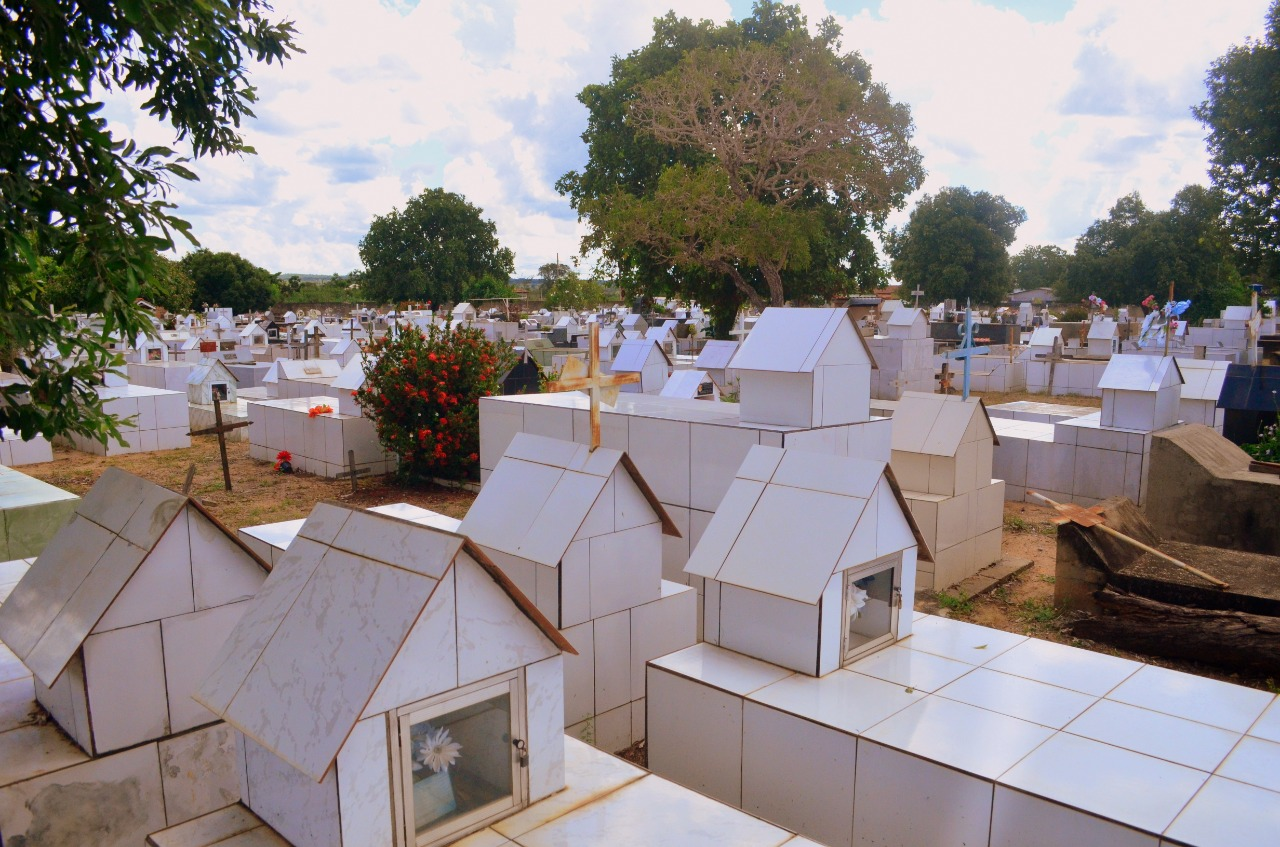
\includegraphics[width=0.5\linewidth]{802.jpeg}
    \caption{Cemitério de Barra das Graças}
    \label{fig:cemi}
\end{figure}

\subsection{Itens e Pistas}

\begin{itemize}
    \item \textbf{Peças Metálicas}: Fragmentos tecnológicos que sugerem que uma criatura alienígena passou por ali.
    \item \textbf{Pegadas com Três Dedos}: Pegadas estranhas indicam a presença de um ser não humano.
    \item \textbf{Entrada Secreta para o Intraterra}: Uma lápide afastada, que ao ser empurrada revela uma entrada para um sistema de túneis subterrâneos.
\end{itemize}

\subsection{Entrada do Intraterra}

Localizada no cemitério, leva à caverna com quatro salas e à Sala do Portal, que está trancada e deve ser monitorada.

\subsection{Cenas de Assombração no Cemitério}

O cemitério de Barra das Garças é palco de estranhas manifestações, especialmente à noite, quando figuras etéreas e sons inquietantes fazem com que poucos se atrevam a cruzar seus portões. Os fantasmas que habitam este lugar têm histórias mal resolvidas, e suas presenças perturbam a paz dos vivos. Abaixo estão três cenas de assombração, cada uma envolvendo um espírito com motivos diferentes para se manifestar.

\subsubsection{O Fantasma do Assassinado – Em Busca de Justiça}

\textbf{Cena:} Enquanto os personagens atravessam uma das alamedas do cemitério, uma figura pálida surge perto de uma lápide isolada. O espírito é de um homem jovem com roupas antigas, rasgadas e manchadas de sangue, olhando para os personagens com uma expressão de tristeza e raiva. Em uma voz baixa e trêmula, ele pede ajuda, dizendo que seu assassinato nunca foi resolvido e que o culpado continua em liberdade. O espírito se aproxima e estende a mão, indicando um lugar específico na cidade onde uma pista crucial para o caso está escondida.

O assassino do fantasma assassinado no cemitério de Barra do Garças foi \index{Bento}Bento Silva, um influente líder local com conexões obscuras. \index{Bento}Bento, conhecido por suas atividades de conspiração com os intraterrenos e pelo uso de notícias falsas para manipular a cidade, cometeu o assassinato para silenciar o fantasma, que havia descoberto sobre seus planos de exploração e aliança com forças sobrenaturais para obter controle da região. 

O fantasma, em vida, era um jornalista chamado \textbf{Joaquim Brandão}, que estava investigando as atividades ilegais de \index{Bento}Bento. Joaquim havia descoberto provas sobre as alianças perigosas que \index{Bento}Bento vinha formando e tinha intenção de publicar uma série de reportagens reveladoras. \index{Bento}Bento, temendo que as informações vazassem e afetassem sua influência, resolveu eliminar o jornalista antes que ele pudesse expor suas conexões.

Mesmo após sua morte, o espírito de Joaquim não conseguiu descansar e ficou preso ao cemitério, buscando uma forma de trazer à tona as provas que \index{Bento}Bento tentou ocultar. Essas pistas e a resolução do mistério do fantasma podem ser descobertas pelos personagens durante a investigação, fornecendo novos elementos sobre as tramas sinistras que envolvem Barra do Garças e os objetivos obscuros de \index{Bento}Bento.

\textbf{Detalhes da Assombração:}
\begin{itemize}
    \item \textbf{Manifestação Visível}: O espírito aparece claramente, mas se desvanece se os personagens se aproximam demais, obrigando-os a manter certa distância para ouvi-lo.
    \item \textbf{Voz Sussurrante}: Ele fala em sussurros, revelando fragmentos de informações sobre seu assassinato, incluindo detalhes que podem indicar o culpado.
    \item \textbf{Pistas Sobrenaturais}: Ao longo da cena, o fantasma indica pontos específicos do cemitério onde podem ser encontrados objetos enterrados ou escondidos – provas esquecidas que podem levar à resolução do caso.
\end{itemize}



\textbf{Objetivo da Cena:} Levar os personagens a investigar o local indicado pelo espírito, encontrando provas que possam ser cruciais para a resolução do crime que tirou a vida do fantasma.

\paragraph{Pistas sobre o Assassinato de Joaquim Brandão}

Durante a investigação, os personagens podem encontrar pistas deixadas pelo fantasma de Joaquim Brandão, que revelam detalhes sobre seu assassinato e a relação entre \index{Bento}Bento Silva e atividades misteriosas em Barra do Garças. Essas pistas ajudam a desvendar o mistério por trás da morte de Joaquim e fornecem evidências contra \index{Bento}Bento.

\begin{itemize}
    \item \textbf{Diário de Joaquim Brandão} - Local: Biblioteca da Cidade  
    O diário de Joaquim Brandão está guardado na seção de arquivos antigos da biblioteca da cidade. Em uma das páginas, Joaquim descreve suspeitas sobre \index{Bento}Bento Silva, mencionando “reuniões noturnas” e "alianças perigosas" que ele estava prestes a expor. A última anotação sugere que ele havia coletado provas e pretendia publicar uma reportagem reveladora.

    \item \textbf{Carta Rasgada} - Local: Escritório do Jornal  
    Nos arquivos do escritório do jornal, onde Joaquim trabalhava, os personagens encontram uma carta rasgada que menciona um “acordo com figuras ocultas” e uma “troca de informações confidenciais” entre \index{Bento}Bento e uma “força subterrânea”. A carta foi endereçada anonimamente a Joaquim, provavelmente como uma advertência para que ele abandonasse a investigação.

    \item \textbf{Relatório de Investigação Incompleto} - Local: Delegacia, Arquivos de Casos Antigos  
    Na delegacia, o escrivão Paulo Farias guardou um relatório de investigação que Joaquim havia submetido para uma possível denúncia contra \index{Bento}Bento. O documento está incompleto e foi arquivado como “pendente” devido ao desaparecimento de Joaquim. No relatório, Joaquim menciona testemunhas e cita locais específicos onde as reuniões de \index{Bento}Bento teriam ocorrido, incluindo o cemitério e um bar local.

    \item \textbf{Gravação de Voz (EVP) do Fantasma} - Local: Cemitério, próximo ao túmulo de Joaquim  
    Durante uma visita noturna ao cemitério, os personagens podem gravar uma mensagem EVP (Electronic Voice Phenomenon) do fantasma de Joaquim. Na gravação, uma voz sussurra a palavra “provas... provas no esconderijo...”. Esta pista leva os personagens a um local secreto onde Joaquim escondeu documentos que comprometeriam \index{Bento}Bento.

    \item \textbf{Fotos Reveladoras} - Local: Subsolo do Bar “Lua Cheia”  
    Joaquim escondeu um conjunto de fotos no subsolo do Bar “Lua Cheia”, onde \index{Bento}Bento realiza algumas de suas reuniões clandestinas. As fotos, tiradas discretamente por Joaquim, mostram \index{Bento}Bento em encontros suspeitos com figuras desconhecidas que têm aparência pálida e vestimentas antigas. Estas fotos são a principal prova de que \index{Bento}Bento mantinha contato direto com forças misteriosas e que eliminou Joaquim para proteger seus segredos.

    \item \textbf{Mapa de Reuniões Noturnas} - Local: Biblioteca da Cidade  
    No arquivo de mapas históricos da cidade, os personagens encontram um mapa anotado por Joaquim, com marcações em áreas onde \index{Bento}Bento e seus associados costumavam se encontrar à noite. Uma das marcações aponta para o cemitério, enquanto outras indicam pontos próximos à Serra do Roncador e ao destacamento do DTCEA-BW. Essas marcações corroboram as suspeitas de Joaquim sobre a natureza perigosa dos encontros de \index{Bento}Bento e revelam pontos estratégicos para investigação.

\end{itemize}

\paragraph{Resumo das Pistas}

Essas pistas, reunidas, revelam que Joaquim estava investigando \index{Bento}Bento Silva e possuía evidências comprometedoras sobre suas ligações com atividades ocultas e figuras misteriosas. A coleta dessas provas permite aos personagens não apenas resolverem o assassinato de Joaquim, mas também entenderem as conexões perigosas que \index{Bento}Bento mantém, levando-os a novos mistérios em Barra do Garças.



\subsubsection{O Espírito da Mãe – Preocupação pela Filha}

\textbf{Cena:} Em uma das áreas mais antigas do cemitério, os personagens sentem uma presença suave e ouvem soluços leves ao longe. Eles se deparam com o espírito de uma mulher de aparência triste e delicada, vestida com roupas antigas e segurando uma fotografia de uma menina pequena, que ela revela ser sua filha. Ela parece aflita, perguntando aos personagens se sabem onde está sua filha, pois não consegue descansar até ter certeza de que ela está bem. A mulher lamenta ter deixado a filha tão jovem e pergunta se os personagens podem verificar se sua menina está em segurança. 

\textbf{Detalhes da Assombração:}
\begin{itemize}
    \item \textbf{Aparição Melancólica}: O espírito aparece com uma expressão de tristeza e ansiedade, segurando a fotografia com delicadeza, como se fosse sua única conexão com o mundo.
    \item \textbf{Toque Gelado}: Quando ela se aproxima dos personagens, eles sentem um frio intenso, como se o desespero dela fosse palpável.
    \item \textbf{Dicas sobre a Filha}: Ao conversarem com o espírito, os personagens percebem que a menina da fotografia é agora a esposa do prefeito, uma mulher que vive em segurança, mas que nunca soube da presença da mãe. 
\end{itemize}

\textbf{Objetivo da Cena:} Dar aos personagens a oportunidade de encontrar um modo de confortar o espírito, seja comunicando-se com a filha ou levando um objeto pessoal dela para assegurar a mãe de que sua filha está em paz.

\subsubsection{O Facínora – Um Espírito Violento e Perigoso}

\textbf{Cena:} Ao se aproximarem de um mausoléu em ruínas, os personagens são subitamente atacados por pedras e pedaços de madeira que parecem ser lançados do nada. O espírito de um homem violento, conhecido em vida por seus crimes, se revela rindo e atacando os personagens sem motivo aparente. Ele tem uma aparência cruel, com um sorriso distorcido e uma postura ameaçadora, quase sólida, e arremessa objetos pesados que podem causar ferimentos graves. O facínora se alimenta do medo e só poderá ser detido por um exorcismo apropriado.

\textbf{Detalhes da Assombração:}
\begin{itemize}
    \item \textbf{Aparição Agressiva}: O espírito surge de forma sólida, tornando-se quase tangível, e tem um rosto desfigurado por uma expressão de fúria e prazer sádico.
    \item \textbf{Objetos em Movimento}: Ele arremessa objetos com uma força impressionante, criando um risco real para os personagens, que precisam se esquivar para evitar ferimentos.
    \item \textbf{Imunidade a Ataques Comuns}: Armas convencionais e tentativas de defesa física são inúteis; o facínora só pode ser repelido com rituais de exorcismo e símbolos sagrados.
\end{itemize}

\textbf{Objetivo da Cena:} Desafiar os personagens a enfrentarem o facínora com métodos sobrenaturais, como orações e símbolos sagrados, para exorcizá-lo e impedir que ele continue aterrorizando o cemitério e colocando vidas em perigo.


\subsection{NPCs}

\begin{itemize}
    \item \textbf{Sr. Carlinhos}: Gerente do Cemitério. Conhecido na cidade por saber todas as histórias do cemitério e compartilhar informações sobre atividades paranormais. Sr. Carlinhos também menciona lendas sobre uma cidade perdida nas redondezas que dizem estar conectada a espíritos obsessores, afirmando que muitas das atividades paranormais podem estar relacionadas a esses espíritos que habitam o local.
\end{itemize}




\section{Igreja de São Miguel}

A Igreja de São Miguel é uma construção imponente de estilo colonial, com uma arquitetura que remonta aos primeiros anos da cidade, carregando uma atmosfera antiga e misteriosa. Esta igreja é um ponto central para a comunidade de Barra das Garças e um local envolto em lendas e histórias sobrenaturais. 

A seguir, uma descrição detalhada dos espaços internos da igreja.

\subsection{Entrada e Foyer}

Ao adentrar a igreja pela grande porta de madeira, os visitantes se deparam com o \textbf{foyer}, um espaço de entrada amplo, com paredes adornadas por imagens religiosas e prateleiras contendo velas que os devotos acendem antes de adentrar o recinto principal. Este ambiente acolhedor introduz o visitante ao ambiente de introspecção que permeia toda a igreja.

\subsection{Nave Central e Pews}

A nave central é o coração da igreja, um longo corredor que se estende até o altar principal. O piso é feito de ladrilhos antigos que, segundo os moradores, contêm traços de mármore vindo de construções antigas. A nave é ladeada por fileiras de \textbf{bancos de madeira} escura, desgastados pelo tempo, onde os fiéis se acomodam para assistir às missas. Entre as fileiras de bancos há pequenas mesas de oração com velas acesas, que criam um ambiente místico, especialmente durante a noite.

\subsection{Capela de Oração Privada}

À esquerda da nave, uma pequena \textbf{capela de oração privada} oferece um espaço mais reservado para orações individuais. A capela é decorada com ícones religiosos menores e velas de cera pura, emitindo uma luz suave e reconfortante. Esse espaço é muitas vezes frequentado por moradores locais que buscam paz interior ou que pretendem se proteger das influências espirituais negativas que rondam a cidade.

\subsection{Sacristia}

Do lado direito da nave, uma porta discreta leva à \textbf{sacristia}, um ambiente pequeno e funcional onde são guardados objetos sagrados, como cálices, crucifixos e vestes utilizadas nas cerimônias. Há também prateleiras cheias de documentos antigos e livros religiosos que podem oferecer pistas sobre fenômenos sobrenaturais. Este espaço é considerado sagrado, e apenas o clero e assistentes podem entrar.

\subsection{Altar e Área do Santuário}

No final da nave central está o \textbf{altar principal}, uma estrutura imponente em madeira esculpida, decorada com estátuas de anjos e santos. Atrás do altar, há uma parede decorada com vitrais que representam São Miguel e outros arcanjos. Durante o dia, a luz que passa por esses vitrais ilumina o altar com um brilho colorido e intenso, dando um aspecto sobrenatural ao ambiente. No centro do altar encontra-se um grande crucifixo, ao lado de velas sempre acesas, símbolo da devoção local.

\subsection{Vitrais e Velas}

Os vitrais ao longo das paredes da igreja são um destaque à parte. Cada vitral conta uma história, desde passagens bíblicas até lendas locais, como o desaparecimento do Coronel Fawcett e as histórias dos intraterrenos. Esses vitrais coloridos permitem que a luz externa adentre o interior da igreja com um brilho difuso, criando sombras misteriosas que amplificam a atmosfera de mistério.

\subsection{Torre do Sino}

No fundo da igreja, há uma escada em espiral que leva até a \textbf{torre do sino}. Esse sino é tocado apenas em ocasiões especiais ou emergências. Da torre, é possível ter uma visão panorâmica da cidade e da Serra do Roncador ao norte. Muitos afirmam que avistamentos de luzes misteriosas no céu são frequentemente observados a partir desta torre.

\subsection{Itens e Pistas na Igreja de São Miguel}

\begin{itemize}
    \item \textbf{Vela com Brilho Azulado}: Uma vela localizada no altar que emite uma luz suave e azulada, semelhante àquela observada no cemitério. Esta vela pode ter ligação com as atividades dos intraterrenos e servir como um ponto de investigação.
    \item \textbf{Livro de Lendas Locais}: Guardado na sacristia, este livro contém relatos sobre a presença de entidades estranhas na região, incluindo espíritos obsessores e histórias sobre a cidade perdida. O livro pode fornecer informações valiosas aos agentes em busca de respostas sobre os fenômenos locais.
\end{itemize}

\subsection{Resumo}

A Igreja de São Miguel é um ponto crucial para a investigação de assombrações em Barra das Garças, proporcionando um ambiente repleto de história, religiosidade e misticismo. Com áreas reservadas e itens sagrados, a igreja serve como um local tanto de proteção quanto de mistério, onde os agentes podem encontrar pistas essenciais para resolver os enigmas que cercam a cidade.


\subsection{NPCs da Igreja de São Miguel}

Abaixo estão descritos os principais personagens que podem interagir com os agentes dentro da Igreja de São Miguel. Cada um possui um papel importante nas atividades da igreja e um histórico pessoal que adiciona profundidade à sua presença na narrativa.

\subsubsection{Sacristão Joaquim dos Santos}

\textbf{Nome:} Joaquim dos Santos  
\textbf{Idade:} 63 anos  
\textbf{Cargo:} Sacristão  
\textbf{Descrição:}  
Joaquim dos Santos é o sacristão responsável pela manutenção da Igreja de São Miguel. Um homem de baixa estatura e semblante sereno, Joaquim veste sempre roupas simples, porém bem cuidadas. Ele tem cabelos grisalhos e uma expressão de bondade, mas carrega uma aura de mistério, resultado de anos convivendo com as lendas e rumores sobrenaturais de Barra das Garças. 

Como sacristão, Joaquim organiza o altar, cuida dos objetos sagrados e prepara os itens necessários para as missas e cerimônias. Ele também se ocupa das velas e dos vitrais, sendo um dos poucos que conhece a história de cada imagem representada neles. Muitos moradores afirmam que ele já presenciou fenômenos estranhos dentro da igreja, mas Joaquim raramente fala sobre isso, a não ser que sinta que a pessoa merece ou precisa saber.

\textbf{Traços de Personalidade:}
\begin{itemize}
    \item \textbf{Sábio e Reservado}: Joaquim prefere observar e ouvir do que falar. Suas respostas são geralmente curtas, mas repletas de significados ocultos.
    \item \textbf{Conhecedor das Lendas}: Ele sabe muito sobre as lendas e mistérios da igreja e da cidade, mas escolhe cuidadosamente com quem compartilha esse conhecimento.
    \item \textbf{Protetor}: Joaquim vê a igreja como um local sagrado e está disposto a defendê-la de qualquer ameaça, incluindo fenômenos sobrenaturais.
\end{itemize}

\textbf{Habilidades e Conhecimentos Especiais:}
\begin{itemize}
    \item \textbf{Conhecimento de Rituais de Proteção}: Joaquim sabe realizar pequenos rituais de proteção e banimento, embora evite utilizá-los abertamente.
    \item \textbf{Percepção Espiritual}: Ele consegue sentir presenças espirituais na igreja e nos arredores, um dom que acredita ter herdado de sua mãe.
    \item \textbf{Artesanato Sagrado}: Joaquim possui habilidade para restaurar e proteger objetos religiosos, mantendo a sacralidade dos itens na igreja.
\end{itemize}



\subsubsection{Diácono Mateus Fontes}

\textbf{Nome:} Mateus Fontes  
\textbf{Idade:} 29 anos  
\textbf{Cargo:} Diácono  
\textbf{Descrição:}  
Mateus Fontes é o jovem diácono da Igreja de São Miguel e braço direito do Padre Anselmo. Ele é um homem alto, com cabelos castanhos e uma expressão amigável, e sua personalidade cativante faz com que seja muito querido entre os fiéis. Diácono Mateus tem uma profunda fé e acredita que sua vocação é proteger e ajudar a comunidade, especialmente diante dos eventos sobrenaturais que ocorrem em Barra das Garças.

Mateus é responsável por auxiliar nas missas, preparar os sacramentos e acompanhar Padre Anselmo nas visitas pastorais. Ele também orienta os jovens da paróquia e organiza grupos de oração para aqueles que enfrentam dificuldades espirituais. Apesar de sua juventude, Mateus é respeitado por sua sabedoria e força espiritual, e está determinado a enfrentar qualquer ameaça à segurança da igreja e da cidade.

\textbf{Traços de Personalidade:}
\begin{itemize}
    \item \textbf{Carismático e Inspirador}: Mateus sabe como motivar e acalmar as pessoas, usando sua fé para trazer esperança.
    \item \textbf{Corajoso e Altruísta}: Ele é destemido e disposto a arriscar-se para proteger sua comunidade.
    \item \textbf{Curioso sobre o Sobrenatural}: Embora seja cético quanto a algumas lendas, Mateus mantém uma mente aberta e está disposto a investigar eventos estranhos que ameacem a paz.
\end{itemize}

\textbf{Habilidades e Conhecimentos Especiais:}
\begin{itemize}
    \item \textbf{Exorcismo e Benção de Espaços}: Mateus conhece rituais de benção e tem treinamento básico em exorcismo, auxiliando Padre Anselmo quando necessário.
    \item \textbf{Conhecimento de Religião e Lendas Locais}: Ele tem um conhecimento sólido sobre teologia, mas também aprendeu lendas locais e está ciente das histórias sobre os intraterrenos.
    \item \textbf{Oratória Persuasiva}: Mateus é capaz de acalmar situações tensas e influenciar outras pessoas, um talento útil em investigações e interações comunitárias.
\end{itemize}

\subsubsection{Padre Anselmo}

\textbf{Nome:} Padre Anselmo Costa  
\textbf{Idade:} 54 anos  
\textbf{Cargo:} Pároco da Igreja de São Miguel  
\textbf{Descrição:}  
Padre Anselmo é o pároco da Igreja de São Miguel, um homem de porte austero e voz tranquila, cuja presença inspira respeito e confiança. Ele é conhecido por sua profunda devoção, sua vasta sabedoria sobre teologia e sua compreensão das histórias e lendas locais de Barra das Garças. Padre Anselmo tem cabelos grisalhos e usa sempre uma batina negra, simbolizando seu compromisso com a fé e o serviço à comunidade.

Por anos, Padre Anselmo ouviu os relatos dos moradores sobre fenômenos estranhos, incluindo visões de luzes e avistamentos de seres incomuns. Ele aconselha cautela aos seus paroquianos e evita fomentar o medo, acreditando que a paz espiritual é a melhor proteção contra influências negativas. Apesar de sua abordagem tranquila, ele leva muito a sério a presença dos chamados espíritos obsessores, que acredita serem entidades que influenciam negativamente certos moradores e eventos na cidade. Padre Anselmo compartilha esses conhecimentos apenas com aqueles que demonstram responsabilidade, incluindo agentes em missões.

\textbf{Traços de Personalidade:}
\begin{itemize}
    \item \textbf{Calmo e Reflexivo}: Padre Anselmo raramente se abala, mantendo-se sereno mesmo em situações difíceis, uma qualidade que o torna um ponto de equilíbrio para a comunidade.
    \item \textbf{Sábio e Prudente}: Ele prefere adotar uma postura de observação e reflexão, evitando confrontos diretos, especialmente com entidades que considera espiritualmente perigosas.
    \item \textbf{Empático e Protetor}: Padre Anselmo demonstra grande compaixão por sua comunidade e está sempre disposto a ajudar aqueles que buscam auxílio espiritual.
\end{itemize}

\textbf{Habilidades e Conhecimentos Especiais:}
\begin{itemize}
    \item \textbf{Conhecimento Profundo das Lendas Locais e Espirituais}: Padre Anselmo conhece em detalhes as histórias dos intraterrenos, espíritos obsessores e outros fenômenos locais, o que o torna uma fonte de informações valiosa.
    \item \textbf{Experiência em Exorcismo e Rituais de Proteção}: Ele é treinado em exorcismo e frequentemente realiza rituais de benção e proteção para moradores e para a igreja. Sua experiência é extensa, e ele sabe lidar com diferentes tipos de manifestações espirituais.
    \item \textbf{Conselheiro Espiritual}: Sua habilidade de aconselhar é acompanhada de uma capacidade de persuasão discreta e inspiradora, o que faz com que as pessoas sintam confiança em suas orientações.
\end{itemize}

\textbf{Histórico e Motivação:}  
Padre Anselmo chegou a Barra das Garças há mais de 20 anos e, desde então, testemunhou mudanças significativas na cidade. Ele acredita que algumas forças espirituais têm se intensificado nos últimos anos e que os fenômenos sobrenaturais na região podem estar ligados a atividades antigas, datando de antes mesmo da fundação da cidade. Seu papel como líder espiritual o motiva a proteger a cidade de influências negativas e a manter a paz entre os moradores. Embora seu foco seja o bem-estar da comunidade, ele entende a importância de estudar essas forças sobrenaturais para proteger melhor aqueles sob sua responsabilidade.

Essas características tornam Padre Anselmo uma figura-chave para os agentes, capaz de oferecer tanto apoio espiritual quanto informações sobre o intraterreno e outras forças misteriosas em Barra das Garças. Seu conhecimento é amplamente respeitado, e ele é um aliado confiável em missões envolvendo investigações espirituais e confrontos sobrenaturais.





\section{Irmandade de São Jerônimo}

A Irmandade de São Jerônimo é uma sociedade religiosa leiga ultraconservadora que se dedica a proteger e preservar os valores e a tradição religiosa da cidade de Barra das Garças. A irmandade foi fundada há várias décadas por imigrantes italianos, e seus membros são conhecidos por sua rigidez em relação aos costumes e moralidade. Eles exercem grande influência na comunidade, inclusive na política local, tendo entre seus membros o vereador Alceu Braga, que utiliza seu cargo para promover as pautas da irmandade.

\subsection{O Prédio da Irmandade}

O edifício da Irmandade de São Jerônimo é um prédio antigo de dois andares, com uma arquitetura que remonta ao período colonial, construído com pedras rústicas e janelas de madeira trabalhada. No interior, o ambiente é austero e decorado com imagens sacras, cruzes e velas que iluminam discretamente os corredores e salas. Em uma das salas, protegida por uma porta de madeira maciça e um cadeado antigo, está a sala de relíquias e registros da irmandade, onde documentos secretos são guardados. A irmandade mantém registros de eventos e atividades de grupos considerados perigosos por eles, além de objetos religiosos que possuem um significado simbólico e espiritual.

A sala de reuniões da irmandade contém uma grande mesa de madeira onde os membros discutem e decidem os rumos da organização. Uma das paredes abriga uma cruz de ferro antiga, que, segundo a tradição, teria sido abençoada por um sacerdote exorcista e utilizada em um ritual de expulsão de espíritos.

\subsection{Personagens da Irmandade}

\paragraph{Vereador Alceu Braga}  
O vereador Alceu é um homem na casa dos 50 anos, com uma postura rígida e conservadora. Alceu é influente na comunidade e utiliza seu cargo para impulsionar projetos de lei que reforçam os valores da irmandade. Ele é visto com desconfiança por grupos religiosos afrodescendentes e figuras políticas progressistas da cidade.

\paragraph{Ancião Giovanni Borelli}  
Com 82 anos, Giovanni é o membro mais antigo e respeitado da irmandade. Ele herdou uma relíquia dos pais, imigrantes italianos que trouxeram um crucifixo de prata, supostamente com poderes de exorcismo. Giovanni é discreto e raramente fala sobre a relíquia, mas é o único que sabe como utilizá-la em rituais de banimento de espíritos. Acredita-se que o crucifixo tenha sido usado em um evento de exorcismo ainda na Itália e, desde então, permaneceu na família.

\paragraph{Padre Júlio, o Conselheiro}  
Padre Júlio, de 64 anos, não é um membro oficial da irmandade, mas participa das reuniões como conselheiro espiritual. Ele é muito respeitado e orienta os membros sobre práticas religiosas. Padre Júlio preza pelo segredo das atividades da irmandade e insiste que os registros de rituais permaneçam sigilosos.

\paragraph{Marco Pereira, o Guardião}  
Marco, de 43 anos, é o responsável pela segurança do prédio da irmandade. Ele garante que ninguém entre nas áreas restritas sem permissão. Marco é um homem discreto, de poucas palavras, e possui um treinamento em autodefesa. Ele guarda a sala de relíquias com grande dedicação e possui um rosário que, segundo ele, protege contra influências malignas.

\paragraph{Ricardo Oliveira, o Escriturário}  
Ricardo é um homem meticuloso, responsável pela manutenção dos arquivos da irmandade. Aos 37 anos, ele mantém uma postura rígida e é extremamente zeloso com os documentos da organização. Ricardo possui um caderno secreto onde registra detalhes de todas as reuniões, mas mantém o conteúdo em segredo até mesmo para seus colegas.

\paragraph{Lucas Mendes, o Noviço}  
Lucas é o membro mais jovem da irmandade, com 24 anos. Ele foi iniciado recentemente e está aprendendo os segredos da organização. Lucas tem uma admiração por Giovanni e deseja aprender sobre o uso da relíquia, mas Giovanni reluta em revelar o segredo do crucifixo.

\section{Religiões Afrodescendentes em Barra das Garças}

Em Barra das Garças, as religiões afro-brasileiras têm uma presença significativa, com três terreiros que acolhem uma parte importante da comunidade. O mais influente deles é o Terreiro de Pai Jorge, conhecido por realizar rituais e cerimônias que atraem fiéis e curiosos da região.

\subsection{Terreiro de Pai Jorge}

O Terreiro de Pai Jorge é o maior e mais respeitado da cidade, fundado por Jorge de Xangô, um sacerdote conhecido por seu conhecimento profundo da Umbanda e do Candomblé. O terreiro é um espaço amplo, cercado por plantas sagradas e decorado com estátuas e elementos que representam os orixás. Pai Jorge é conhecido por seus rituais poderosos e por sua sabedoria espiritual, além de ser guardião de alguns segredos espirituais importantes para a comunidade.

\paragraph{Pai Jorge de Xangô}  
Líder espiritual do terreiro, Pai Jorge, de 58 anos, é um respeitado sacerdote com habilidades reais em magia branca. Ele possui uma forte conexão com o orixá Xangô e é capaz de realizar rituais de proteção e cura que possuem efeitos notáveis. Pai Jorge é o conselheiro de muitos moradores e mantém um bastão sagrado, utilizado em rituais específicos de benção e purificação.

\paragraph{Mãe Cleonice, a Curandeira}  
Mãe Cleonice, de 62 anos, é uma mulher de grande conhecimento herbal e ajuda a comunidade com ervas e poções de cura. Ela é responsável pela preparação dos banhos e infusões que ajudam nas práticas espirituais do terreiro. Cleonice guarda consigo um amuleto abençoado pelo orixá Oxum, que dizem trazer sorte e prosperidade para quem o possui.

\paragraph{Joaquim, o Ogã}  
Joaquim é o ogã do terreiro, responsável pela música e pelos cânticos sagrados durante as cerimônias. Aos 45 anos, Joaquim é hábil no uso do atabaque e possui um colar que representa a proteção do orixá Ogum. Ele é considerado um defensor espiritual do terreiro e está sempre presente para apoiar os rituais de Pai Jorge.

\paragraph{Luciana, a Filha de Santo}  
Com 30 anos, Luciana é uma filha de santo de Pai Jorge, devota de Iemanjá. Ela participa dos rituais de purificação e proteção e auxilia nas cerimônias. Luciana possui um espelho sagrado, presente de Mãe Cleonice, que utiliza em rituais de meditação e fortalecimento espiritual.

\paragraph{Terreiros Menores}

Além do Terreiro de Pai Jorge, há outros dois terreiros em Barra das Garças:

\subsubsection{Terreiro de Mãe Celina}  
Um terreiro menor, mas ativo, liderado por Mãe Celina, que realiza rituais de purificação e consultas espirituais.

\subsubsection{Terreiro de Pai Ernesto}  
Conhecido por seus rituais noturnos, Pai Ernesto é um sacerdote que ajuda os moradores a resolver problemas pessoais e espirituais por meio das práticas religiosas afro-brasileiras.

\section{Outras Igrejas de Barra das Garças}

Além da Igreja de São Miguel, existem outras duas pequenas igrejas na cidade, cada uma com suas particularidades e liderança.

\subsection{Igreja de Santa Clara}

A Igreja de Santa Clara é uma pequena capela localizada no bairro mais antigo da cidade. É uma construção modesta, mas frequentada por uma comunidade fiel.

\paragraph{Padre Carlos}  
O responsável pela Igreja de Santa Clara, Padre Carlos, é um homem de 55 anos, com uma abordagem acolhedora e humilde. Ele é conhecido por sua proximidade com a comunidade e por oferecer apoio espiritual para todos os que procuram a igreja. Padre Carlos possui um crucifixo de prata que foi presente de sua avó e acredita que o objeto é abençoado.

\paragraph{Sacristão Antônio}  
Antônio é o sacristão de 46 anos que cuida da igreja com zelo. Ele é tímido e reservado, mas extremamente devoto e leal a Padre Carlos. Antônio guarda um pequeno relicário de Santa Clara, que ele afirma proteger a igreja de más influências.

\subsection{Capela de Nossa Senhora das Dores}

A Capela de Nossa Senhora das Dores é um templo discreto e pacífico, cercado por um jardim bem cuidado. A capela é administrada por Padre Francisco, que realiza missas semanais e acolhe fiéis de toda a cidade.

\paragraph{Padre Francisco}  
Padre Francisco, de 60 anos, é um religioso experiente, com uma postura serena e compassiva. Ele dedica-se à orientação espiritual dos fiéis e realiza visitas constantes às famílias da região. O padre possui um rosário que, segundo ele, já foi utilizado em uma bênção especial, o que lhe confere uma energia protetora.

\paragraph{Sacristão Paulo}  
Paulo é um jovem de 28 anos que auxilia Padre Francisco nas atividades da capela. Ele é conhecido por sua devoção e entusiasmo. Paulo possui um livro antigo de orações, passado de geração em geração em sua família


\section{Comunidades Evangélicas em Barra das Garças}

Em Barra das Garças, as comunidades evangélicas são diversas e incluem várias denominações com templos espalhados por toda a cidade. Cada corrente possui suas próprias doutrinas e modos de adoração, refletindo a diversidade de interpretações e práticas dentro do protestantismo. Abaixo, descrevemos quatro correntes evangélicas representativas na cidade, cada uma com seus templos e líderes.

\subsection{Igreja do Caminho da Fé}

A Igreja do Caminho da Fé é uma das congregações evangélicas mais tradicionais da cidade, com uma doutrina voltada para o estudo bíblico e a promoção de valores familiares. O templo principal é grande e possui um auditório com capacidade para centenas de pessoas, decorado de maneira simples e funcional, com ênfase na palavra e na comunhão.

\paragraph{Pastor Eduardo Reis}  
Pastor Eduardo é um líder respeitado, com um forte compromisso com a comunidade e um estilo de vida modesto. Ele é conhecido por suas pregações baseadas na caridade e na justiça social, realizando projetos de assistência para os necessitados da cidade. Eduardo promove cursos de formação bíblica e incentiva a participação dos jovens na igreja, buscando construir uma comunidade unida e altruísta. Sua abordagem caridosa e sincera faz dele uma figura admirada até mesmo fora do meio evangélico.

\subsection{Comunidade Esperança Celestial}

A Comunidade Esperança Celestial é uma igreja pentecostal que valoriza o louvor e a experiência espiritual intensa em suas celebrações. Seus cultos incluem cânticos animados, orações em grupo e eventos de evangelização. O templo é decorado com cores vivas e possui uma grande cruz iluminada no altar, sendo o principal ponto de encontro da comunidade para cultos semanais e eventos especiais.

\paragraph{Pastor Miguel Rocha}  
Pastor Miguel é um líder carismático e reconhecido por suas habilidades de comunicação. Sua pregação é enérgica, e ele é conhecido por enfatizar a importância da fé para a conquista de milagres e bênçãos na vida pessoal e familiar de seus fiéis. Embora seja visto como um pastor “normal”, Pastor Miguel é cuidadoso em suas ações e não se envolve em polêmicas, mantendo um bom relacionamento com os fiéis e com as outras lideranças religiosas da cidade.

\subsection{Templo da Prosperidade Divina}

O Templo da Prosperidade Divina é uma congregação de doutrina neopentecostal, focada em temas de prosperidade financeira e “batalha espiritual”. O templo é grandioso, com equipamentos de som e luz modernos, e ostenta uma fachada imponente que chama atenção. Os cultos enfatizam o poder da doação para a obtenção de bênçãos e prosperidade.

\paragraph{Pastor Osvaldo Santos}  
Pastor Osvaldo é uma figura polêmica na cidade, frequentemente criticado por sua insistência em campanhas de doação de altos valores e promessas de retorno financeiro divino para os fiéis. Ele vive de forma ostensiva, com roupas e acessórios de luxo, o que levanta suspeitas entre a população sobre a real destinação das doações. Muitos acreditam que Pastor Osvaldo explora a fé dos fiéis, e há rumores de que ele está envolvido em esquemas financeiros. Apesar das críticas, ele mantém uma base fiel de seguidores e justifica seu estilo de vida como resultado das “bênçãos de Deus”.

\subsection{Igreja Batista do Vale}

A Igreja Batista do Vale é uma congregação discreta e acolhedora, com um estilo de adoração mais tranquilo e um forte foco em projetos sociais. O templo é simples, mas bem cuidado, com uma pequena biblioteca e um espaço para atividades de estudo bíblico e recreação para crianças e jovens. A igreja é conhecida por suas campanhas de ajuda aos mais necessitados e seu envolvimento em atividades de responsabilidade social.

\paragraph{Pastor Roberto Silva}  
Pastor Roberto é um homem dedicado e responsável, que guia a igreja de maneira serena e comedida. Ele é um líder respeitado, embora mantenha um perfil discreto e reservado. Pastor Roberto se dedica ao estudo bíblico e incentiva os fiéis a buscar uma vida de retidão e serviço à comunidade. Ele promove cursos de formação cristã e programas de apoio à juventude. Como líder, Pastor Roberto é visto como “normal”, uma presença constante e confiável para a comunidade batista do bairro.

\subsection{Visão Geral das Correntes Evangélicas}

Cada uma dessas comunidades representa um segmento da diversidade evangélica na cidade, com abordagens distintas em relação à fé e à forma de conduzir o templo. Enquanto a Igreja do Caminho da Fé se destaca pelo compromisso social de Pastor Eduardo, a Comunidade Esperança Celestial é um centro de adoração vibrante e acolhedor. Em contraste, o Templo da Prosperidade Divina levanta questões de ética e sinceridade nas práticas de Pastor Osvaldo, atraindo tanto fiéis quanto críticas pela ênfase em doações. Já a Igreja Batista do Vale destaca-se pelo trabalho comunitário, uma característica prezada por Pastor Roberto e seus seguidores.

Essas diferenças refletem as várias facetas das comunidades evangélicas em Barra das Garças, que coexistem apesar de suas diferenças, oferecendo opções distintas de adoração e práticas religiosas para a população local.

\section{O Coven de Ágata Negra e Suas Bruxas}

Escondido nos limites de Barra das Garças, o Coven de Ágata Negra é um círculo de bruxas conhecidas por práticas esotéricas e conhecimentos antigos. Elas se reúnem em uma clareira na floresta, em noites de lua cheia, para rituais que conectam suas forças à natureza e aos elementos. O coven é formado por cinco bruxas, cada uma com habilidades únicas, que, unidas, criam uma forte presença mística na região.

\subsection{A Sede do Coven}

A sede do coven, conhecida como ``Casa de Ágata Negra'', é uma cabana rústica e oculta, cercada por árvores antigas e flora densa. Com velas e amuletos pendurados nas janelas, a casa parece distante da cidade, tanto física quanto espiritualmente. Dentro, o ambiente é decorado com objetos ritualísticos: cristais, ervas secas e livros de feitiçaria. Um altar no centro da sala é dedicado à deusa da natureza, com oferendas de flores, frutas e pequenos animais esculpidos em madeira.

\subsection{As Bruxas do Coven}

\paragraph{Helena, a Matriarca}  
Helena é a bruxa mais velha e respeitada do coven, conhecida como a matriarca. Ela possui vasto conhecimento sobre plantas medicinais e poções curativas. Helena também é guardiã de um grimório ancestral, passado de geração em geração, que contém feitiços poderosos de proteção e cura. Sua presença imponente inspira confiança e respeito entre as outras bruxas.

\paragraph{Mara, a Visionária}  
Mara é uma jovem bruxa com habilidades visionárias, capaz de realizar premonições e leituras de cartas com impressionante precisão. Seu poder intuitivo lhe permite prever acontecimentos futuros, e ela frequentemente guia o coven sobre decisões importantes. Embora seja reservada, sua sabedoria mística é valiosa para o grupo.

\paragraph{Selena, a Guardiã dos Espíritos}  
Selena é uma bruxa de meia-idade com habilidades de comunicação com espíritos. Ela serve como mediadora entre o mundo dos vivos e o dos mortos, realizando rituais de proteção e purificação. Selena é conhecida por seus amuletos protetores e práticas de exorcismo, sendo procurada por pessoas que acreditam estar sendo assombradas.

\paragraph{Bianca, a Feiticeira Elemental}  
Bianca é uma bruxa hábil em manipular os elementos, especialmente a água e o fogo. Seus feitiços são conhecidos por sua intensidade e precisão. Bianca é responsável pelos rituais ligados à natureza e à renovação, sendo uma figura essencial durante as celebrações de solstícios e equinócios. Ela possui um bastão encantado que utiliza para canalizar sua energia elemental.

\paragraph{Isabel, a Aprendiz}  
Isabel é a mais nova do grupo e aprendiz do coven. Embora inexperiente, ela demonstra grande aptidão para feitiços de cura e proteção. Isabel está sob a orientação direta de Helena, aprendendo as tradições e práticas da magia ancestral. Sua curiosidade e determinação a tornam uma promessa para o futuro do coven.

\subsection{Segredos e Rituais}

O coven guarda alguns segredos que são conhecidos apenas por suas integrantes. Um desses segredos envolve a ``Relíquia de Ágata'', uma pedra negra com propriedades místicas, que dizem ser a chave para aumentar os poderes de cura de quem a possui. Helena é a guardiã dessa relíquia e utiliza-a em ocasiões especiais para fortalecer os rituais de proteção.

Outro segredo é o ``Feitiço da Nuvem Sombria'', um ritual poderoso que o coven utiliza em casos de extrema necessidade para proteger a comunidade de forças negativas. Esse feitiço é raro e demanda grande energia das bruxas, sendo reservado apenas para momentos críticos.

\subsection{Rituais e Festividades}

O coven celebra regularmente as mudanças de estação e as fases da lua, com destaque para os solstícios e equinócios. Esses eventos são oportunidades de renovação espiritual, nos quais as bruxas realizam rituais para agradecer à natureza e reforçar seus laços com o ambiente. As festividades são momentos de união, onde cada bruxa contribui com seu dom único, fortalecendo os laços do grupo e renovando o poder coletivo do coven.

Com o tempo, o Coven de Ágata Negra tem se tornado uma lenda em Barra das Garças, uma presença oculta e poderosa, cercada por mistérios e reverência. Suas bruxas, com habilidades distintas e complementares, formam um grupo que preserva o conhecimento ancestral, transmitindo-o de geração em geração e protegendo a comunidade dos perigos invisíveis do mundo místico.

